\documentclass{standalone}
\usepackage{tikz}
\usetikzlibrary{patterns, positioning}

\begin{document}
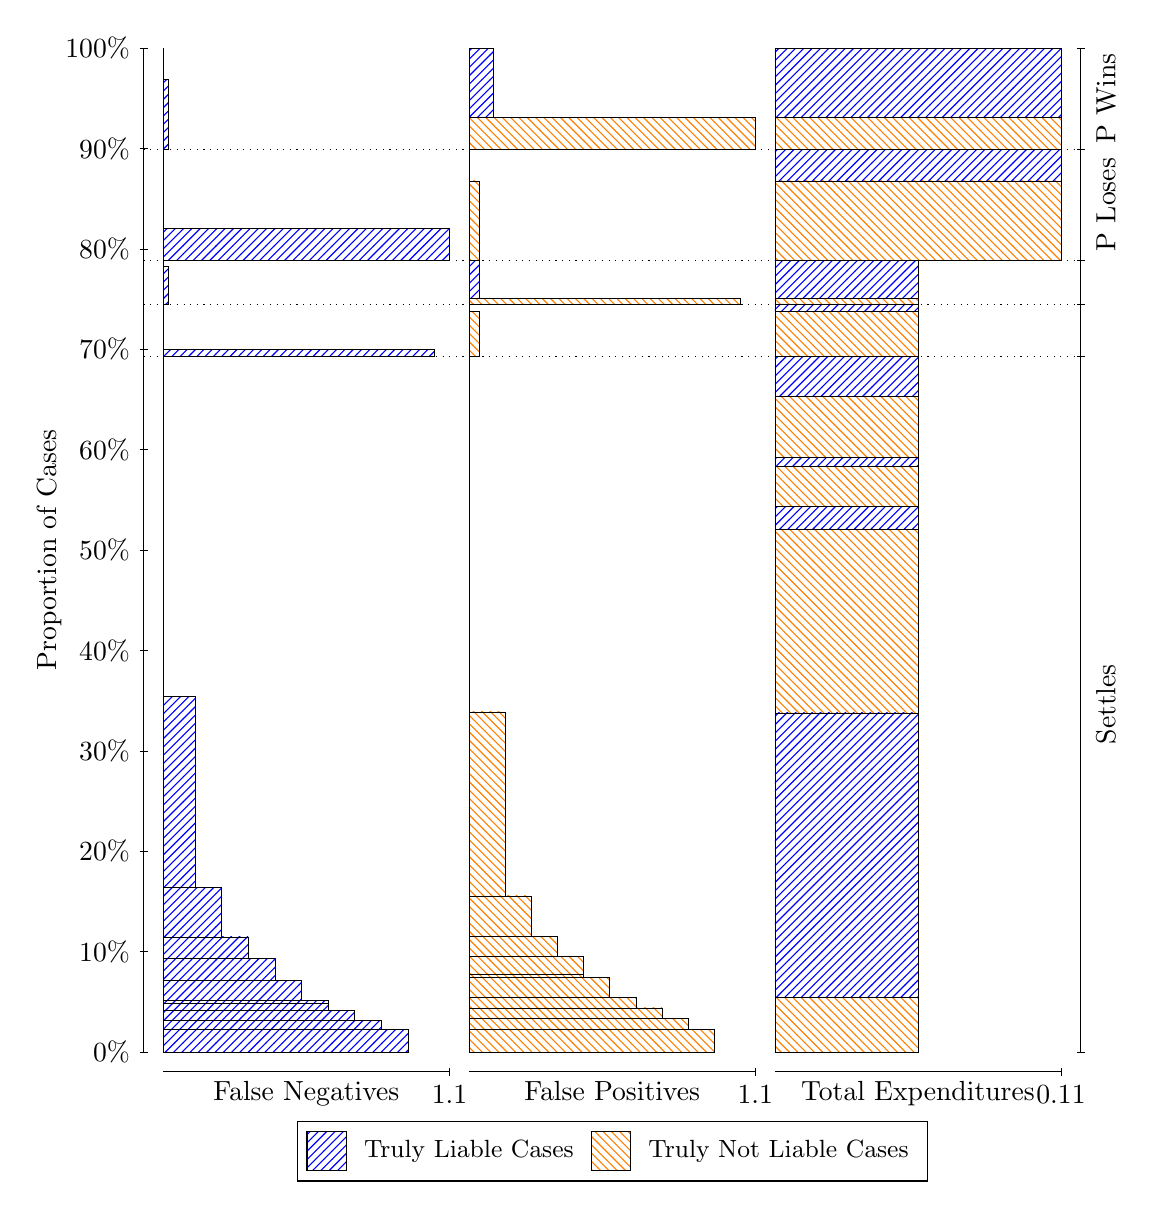
\begin{tikzpicture}
\draw[black, very thin] (1.5,1.75) -- (1.5,14.5);
\node[rotate=90, anchor=center] at (0.3, 8.125) {Proportion of Cases};
\draw[black, very thin] (1.45,1.75) -- (1.55,1.75);
\node[anchor=east] at (1.45, 1.75) {0\%};
\draw[black, very thin] (1.45,3.025) -- (1.55,3.025);
\node[anchor=east] at (1.45, 3.025) {10\%};
\draw[black, very thin] (1.45,4.3) -- (1.55,4.3);
\node[anchor=east] at (1.45, 4.3) {20\%};
\draw[black, very thin] (1.45,5.575) -- (1.55,5.575);
\node[anchor=east] at (1.45, 5.575) {30\%};
\draw[black, very thin] (1.45,6.85) -- (1.55,6.85);
\node[anchor=east] at (1.45, 6.85) {40\%};
\draw[black, very thin] (1.45,8.125) -- (1.55,8.125);
\node[anchor=east] at (1.45, 8.125) {50\%};
\draw[black, very thin] (1.45,9.4) -- (1.55,9.4);
\node[anchor=east] at (1.45, 9.4) {60\%};
\draw[black, very thin] (1.45,10.675) -- (1.55,10.675);
\node[anchor=east] at (1.45, 10.675) {70\%};
\draw[black, very thin] (1.45,11.95) -- (1.55,11.95);
\node[anchor=east] at (1.45, 11.95) {80\%};
\draw[black, very thin] (1.45,13.225) -- (1.55,13.225);
\node[anchor=east] at (1.45, 13.225) {90\%};
\draw[black, very thin] (1.45,14.5) -- (1.55,14.5);
\node[anchor=east] at (1.45, 14.5) {100\%};

\draw[black, very thin] (13.4,1.75) -- (13.4,14.5);
\draw[black, very thin] (13.35,1.75) -- (13.45,1.75);
\node[anchor=west] at (13.35, 1.75) {};
\draw[black, very thin] (13.35,10.585) -- (13.45,10.585);
\node[anchor=west] at (13.35, 10.585) {};
\draw[black, very thin] (13.35,11.241) -- (13.45,11.241);
\node[anchor=west] at (13.35, 11.241) {};
\draw[black, very thin] (13.35,11.807) -- (13.45,11.807);
\node[anchor=west] at (13.35, 11.807) {};
\draw[black, very thin] (13.35,13.216) -- (13.45,13.216);
\node[anchor=west] at (13.35, 13.216) {};
\draw[black, very thin] (13.35,14.5) -- (13.45,14.5);
\node[anchor=west] at (13.35, 14.5) {};

\draw[black, very thin, pattern color=blue, pattern=north east lines] (1.75,1.75) rectangle (4.8552,2.0322);
\draw[black, very thin, pattern color=blue, pattern=north east lines] (1.75,2.0322) rectangle (4.5172,2.1504);
\draw[black, very thin, pattern color=blue, pattern=north east lines] (1.75,2.1504) rectangle (4.1793,2.2772);
\draw[black, very thin, pattern color=blue, pattern=north east lines] (1.75,2.2772) rectangle (3.8413,2.3641);
\draw[black, very thin, pattern color=blue, pattern=north east lines] (1.75,2.3641) rectangle (3.8413,2.4035);
\draw[black, very thin, pattern color=blue, pattern=north east lines] (1.75,2.4035) rectangle (3.5033,2.6552);
\draw[black, very thin, pattern color=blue, pattern=north east lines] (1.75,2.6552) rectangle (3.1653,2.9356);
\draw[black, very thin, pattern color=blue, pattern=north east lines] (1.75,2.9356) rectangle (2.8273,3.2109);
\draw[black, very thin, pattern color=blue, pattern=north east lines] (1.75,3.2109) rectangle (2.4893,3.8358);
\draw[black, very thin, pattern color=blue, pattern=north east lines] (1.75,3.8358) rectangle (2.1514,6.2647);
\draw[black, very thin, pattern color=orange, pattern=north west lines] (1.75,6.2647) rectangle (1.75,10.585);
\draw[black, very thin, pattern color=blue, pattern=north east lines] (1.75,10.585) rectangle (5.1932,10.672);
\draw[black, very thin, pattern color=orange, pattern=north west lines] (1.75,10.672) rectangle (1.75,11.241);
\draw[black, very thin, pattern color=blue, pattern=north east lines] (1.75,11.241) rectangle (1.8134,11.729);
\draw[black, very thin, pattern color=orange, pattern=north west lines] (1.75,11.729) rectangle (1.75,11.807);
\draw[black, very thin, pattern color=blue, pattern=north east lines] (1.75,11.807) rectangle (5.3833,12.21);
\draw[black, very thin, pattern color=orange, pattern=north west lines] (1.75,12.21) rectangle (1.75,13.216);
\draw[black, very thin, pattern color=blue, pattern=north east lines] (1.75,13.216) rectangle (1.8134,14.098);
\draw[black, very thin, pattern color=orange, pattern=north west lines] (1.75,14.098) rectangle (1.75,14.5);
\draw[black, very thin, pattern color=orange, pattern=north west lines] (5.6333,1.75) rectangle (8.7476,2.0354);
\draw[black, very thin, pattern color=orange, pattern=north west lines] (5.6333,2.0354) rectangle (8.4154,2.1737);
\draw[black, very thin, pattern color=orange, pattern=north west lines] (5.6333,2.1737) rectangle (8.0832,2.3111);
\draw[black, very thin, pattern color=orange, pattern=north west lines] (5.6333,2.3111) rectangle (7.751,2.4458);
\draw[black, very thin, pattern color=orange, pattern=north west lines] (5.6333,2.4458) rectangle (7.4189,2.6983);
\draw[black, very thin, pattern color=orange, pattern=north west lines] (5.6333,2.6983) rectangle (7.0867,2.741);
\draw[black, very thin, pattern color=orange, pattern=north west lines] (5.6333,2.741) rectangle (7.0867,2.9622);
\draw[black, very thin, pattern color=orange, pattern=north west lines] (5.6333,2.9622) rectangle (6.7545,3.2217);
\draw[black, very thin, pattern color=orange, pattern=north west lines] (5.6333,3.2217) rectangle (6.4223,3.7311);
\draw[black, very thin, pattern color=orange, pattern=north west lines] (5.6333,3.7311) rectangle (6.0901,6.0701);
\draw[black, very thin, pattern color=blue, pattern=north east lines] (5.6333,6.0701) rectangle (5.6333,10.585);
\draw[black, very thin, pattern color=orange, pattern=north west lines] (5.6333,10.585) rectangle (5.7579,11.154);
\draw[black, very thin, pattern color=blue, pattern=north east lines] (5.6333,11.154) rectangle (5.6333,11.241);
\draw[black, very thin, pattern color=orange, pattern=north west lines] (5.6333,11.241) rectangle (9.0798,11.32);
\draw[black, very thin, pattern color=blue, pattern=north east lines] (5.6333,11.32) rectangle (5.7579,11.807);
\draw[black, very thin, pattern color=orange, pattern=north west lines] (5.6333,11.807) rectangle (5.7579,12.813);
\draw[black, very thin, pattern color=blue, pattern=north east lines] (5.6333,12.813) rectangle (5.6333,13.216);
\draw[black, very thin, pattern color=orange, pattern=north west lines] (5.6333,13.216) rectangle (9.2667,13.618);
\draw[black, very thin, pattern color=blue, pattern=north east lines] (5.6333,13.618) rectangle (5.9448,14.5);
\draw[black, very thin, pattern color=orange, pattern=north west lines] (9.5167,1.75) rectangle (11.333,2.4458);
\draw[black, very thin, pattern color=blue, pattern=north east lines] (9.5167,2.4458) rectangle (11.333,6.0553);
\draw[black, very thin, pattern color=orange, pattern=north west lines] (9.5167,6.0553) rectangle (11.333,8.3943);
\draw[black, very thin, pattern color=blue, pattern=north east lines] (9.5167,8.3943) rectangle (11.333,8.6765);
\draw[black, very thin, pattern color=orange, pattern=north west lines] (9.5167,8.6765) rectangle (11.333,9.1859);
\draw[black, very thin, pattern color=blue, pattern=north east lines] (9.5167,9.1859) rectangle (11.333,9.3041);
\draw[black, very thin, pattern color=orange, pattern=north west lines] (9.5167,9.3041) rectangle (11.333,10.08);
\draw[black, very thin, pattern color=blue, pattern=north east lines] (9.5167,10.08) rectangle (11.333,10.585);
\draw[black, very thin, pattern color=orange, pattern=north west lines] (9.5167,10.585) rectangle (11.333,11.154);
\draw[black, very thin, pattern color=blue, pattern=north east lines] (9.5167,11.154) rectangle (11.333,11.241);
\draw[black, very thin, pattern color=orange, pattern=north west lines] (9.5167,11.241) rectangle (11.333,11.32);
\draw[black, very thin, pattern color=blue, pattern=north east lines] (9.5167,11.32) rectangle (11.333,11.807);
\draw[black, very thin, pattern color=orange, pattern=north west lines] (9.5167,11.807) rectangle (13.15,12.813);
\draw[black, very thin, pattern color=blue, pattern=north east lines] (9.5167,12.813) rectangle (13.15,13.216);
\draw[black, very thin, pattern color=orange, pattern=north west lines] (9.5167,13.216) rectangle (13.15,13.618);
\draw[black, very thin, pattern color=blue, pattern=north east lines] (9.5167,13.618) rectangle (13.15,14.5);
\draw[black, dotted] (1.5,10.585) -- (13.4,10.585);
\draw[black, dotted] (1.5,11.241) -- (13.4,11.241);
\draw[black, dotted] (1.5,11.807) -- (13.4,11.807);
\draw[black, dotted] (1.5,13.216) -- (13.4,13.216);
\draw[black, very thin] (1.75,1.5) -- (5.3833,1.5);
\node[anchor=north] at (3.5667, 1.5) {False Negatives};
\draw[black, very thin] (5.3833,1.45) -- (5.3833,1.55);
\node[anchor=north] at (5.3833, 1.45) {1.1};

\draw[black, very thin] (5.6333,1.5) -- (9.2667,1.5);
\node[anchor=north] at (7.45, 1.5) {False Positives};
\draw[black, very thin] (9.2667,1.45) -- (9.2667,1.55);
\node[anchor=north] at (9.2667, 1.45) {1.1};

\draw[black, very thin] (9.5167,1.5) -- (13.15,1.5);
\node[anchor=north] at (11.333, 1.5) {Total Expenditures};
\draw[black, very thin] (13.15,1.45) -- (13.15,1.55);
\node[anchor=north] at (13.15, 1.45) {0.11};

\node[black, centered, rotate=90] at (13.72, 6.1674) {Settles};


\node[black, centered, rotate=90] at (13.72, 12.511) {P Loses};
\node[black, centered, rotate=90] at (13.72, 13.858) {P Wins};

\draw (7.449999999999999,1.5) node[draw=none] (baseCoordinate) {};
\begin{scope}[align=center]
        \matrix[scale=0.5, draw=black, below=0.5cm of baseCoordinate, nodes={draw}, column sep=0.1cm]{
            \node[rectangle, draw, minimum width=0.5cm, minimum height=0.5cm, pattern=north east lines, pattern color=blue] {}; &
            \node[draw=none, font=\small] (B) {Truly Liable Cases}; &
            \node[rectangle, draw, minimum width=0.5cm, minimum height=0.5cm, pattern=north west lines, pattern color=orange] {}; &
            \node[draw=none, font=\small] (B) {Truly Not Liable Cases}; \\
            };
\end{scope}

\end{tikzpicture}
\end{document}